\subsection{Bayesian Linear Regression}\label{ssec:regression}

\begin{figure*}[t]
    \centering
    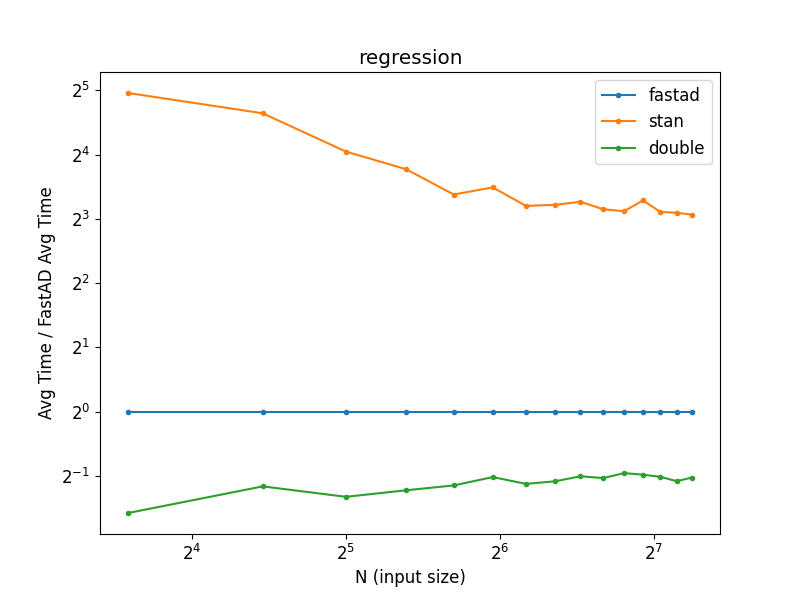
\includegraphics[width=\textwidth]{figs/regression_fig.png}
    \caption{%
        Bayesian linear regression benchmark of Stan against FastAD 
        plotted relative to FastAD average time.
    }\label{fig:regression}
\end{figure*}

This section marks the first macro-benchmark example.
We consider the following Bayesian linear regression model:
\begin{align*}
    y &\sim N\paren{X\cdot w + b, \sigma^2} \\
    w &\sim N\paren{0,1} \\
    b &\sim N\paren{0,1} \\
    \sigma &\sim Unif\paren{0.1, 10.}
\end{align*}
The target function is the log of the joint probability density function (up to a constant).
For this benchmark, we only consider Stan since they specialize in differentiating such functions
and because the other libraries were not well-suited to implement this efficiently.
The fill function for this functor will resize a vector of size $N = 2^K$ as $\tilde{N} = (K + 1) \cdot 10 + 2$,
where the first $(K+1) \cdot 10$ values refer to $w$ and the rest refer to $b$ and $\sigma$, respectively.
It also resizes its private members $y \in \R^{1000}$ and $X \in \R^{1000 \times \tilde{N}}$, which are constants.
All quantities are randomly generated uniformly in $(-1,1)$ range,
but $\sigma$ modified to be strictly positive.

FastAD outperforms Stan by 8 times for the largest $N$.
The trend stabilizes starting from around $N=70$.
It is interesting to see that FastAD is only 2 times slower than the baseline,
despite the model consisting of a large matrix multiplication and many normal log-pdf functions.
One of the reasons is that the compiler was able to optimize-out backward-evaluation for $X$, 
since constants implement a no-op for backward-evaluation.
If we assume that the most expensive operation is the matrix multiplication,
AD evaluation approximately takes 2 matrix multiplication between a matrix and a vector.
We can then approximate a lower bound for manually-written gradient computation to be two times the baseline.
The relative time of FastAD to this approximation is
$1.018$, implying less than $ 1.8\%$ overhead from a manually-written code.
